% !TeX spellcheck = en_GB


\chapter{Appendix Metrics}
\pagenumbering{gobble} 
\label{appendix:metrics}

	A fundamental part of a machine learning project consists of evaluating the performance. There are plenty of metrics to carry out this evaluation and the results will look in one way or another depending on the method utilized. The following two are the most used in this project
	
\section*{Classification Accuracy}

	This is a technique commonly used and it is usually referred to as accuracy. It can be defined as the relationship between the amount of right predictions and the total number on input instances \cite{Scikit-learn}.
	% Formula of accuracy
	\[
	\ \ acc = \frac{Number\ of\ incorrect\  predictions}{Number\ of\ total\ input\ instances}
	\]
	
	This metric is appropriate when dealing with a balanced dataset, i.e., the same of number of samples per class.
	If the problem being addressed deals with unbalanced data, then the accuracy value could be a higher value due to predict all the instances belong to the major class. For example, if $90\%$ of the data are part of the same class A and the model predictions are for this class, then the accuracy value will be $90\%$, which apparently is a satisfying output, even though we are misclassifying all the samples from class B \cite{Mishra2018} and the system is not learning. 
	
\section*{Confusion matrix}

		% Confusion matrix exmaple
	\begin{figure}[b]
		\centering
		\captionsetup{justification=centering}
		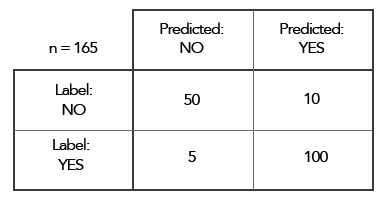
\includegraphics[scale=0.6]{confusion-matrix}
		\caption{Example of confusion matrix}
		\label{fig:mesh6}
	\end{figure}

	As it own name indicates, the output of this type of metric consists on a matrix that shows a complete evaluation of the model. By definition, an entry $i,j$ of the matrix denotes the amount of observations that belong to group $i$ but are predicted as group $j$ \cite{Scikit-learn}. For example, considering a binary classification problem in which there are two classes, YES and NO, for a test set composed by 165 samples, the matrix included in figure \ref{fig:mesh6} is obtained. 
	
	There are four groups that can be extracted from this matrix: True positives, the samples that are predicted as YES and that is in fact their true label, True Negatives, those cases that were predicted as NO and they are originally labelled as NO, False Positives, in which the predicted label is YES but they are actually negative, and False Negatives, those in which the predicted label is NO when their original label is YES.
	
	This metric an the one explained before, accuracy, can be related by taking the diagonal of the matrix and computing the next operation:
	
	\[
	\ \ acc = \frac{TruePositives +\ FalseNegatives}{Total\ number\ of\ samples} = 
	\ \ \frac{100 +\ 50}{165} = 0.91
	\]
	
	When the classification task consists on more than two classes, a multiclass problem, a similar definition of the confusion matrix can be extended from the binary problem. Considering a certain observation $C_k$, the True positive part of the matrix is placed in the exact point where the column and the row of this certain observation are crossed, i.e, when the predicted label is equal to the true label. The False positives samples are placed along the column $C_k$ for all the rows $C_0, ..., C_{k-1}, C{k+1}, ..., C_n$ which refers to all the samples that have been misclassified as the class $C_k$. The False negatives are, however, all the samples that originally are originally labelled as $C_k$ but have been wrongly categorized as $C_0, ..., C_{k-1}, C{k+1}, ..., C_n$ classes. Finally, the True negative samples are distributed across all the other positions in the matrix. In figure \ref{fig:mesh9}, an example for this explanation is shown.
	
	\begin{figure}[h]
		\centering
		\captionsetup{justification=centering}
		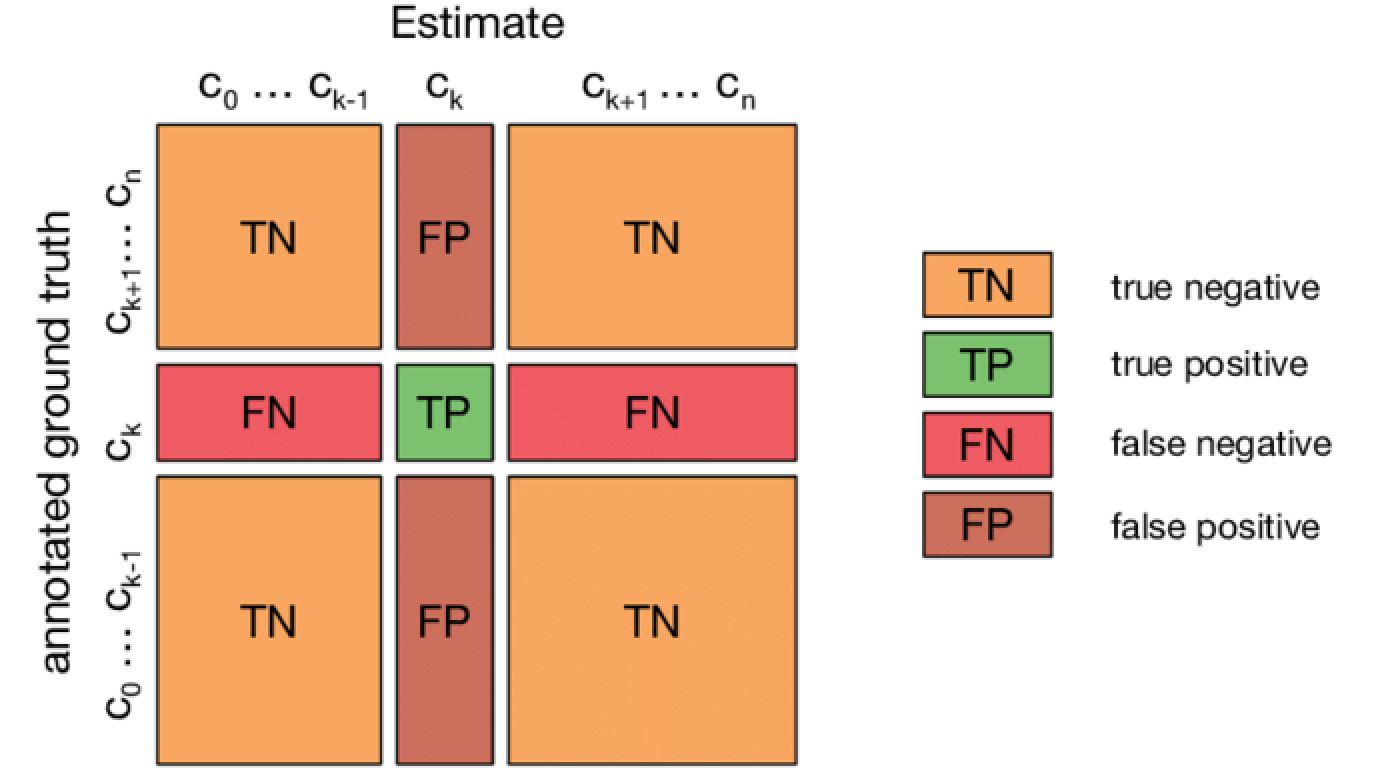
\includegraphics[scale=0.4]{conf-mat-multi}
		\caption{Confusion matrix for a multiclass classification \cite{Kruger2018}}
		\label{fig:mesh9}
	\end{figure}
	
\chapter{Appendix k-Fold Cross Validation}
\pagenumbering{gobble}
\label{appendix:kfold}

	The cross-validation technique is a resampling practice that is commonly used in order to evaluate machine learning algorithms when the dataset is not very large. It just depends on the parameter $k$ which represents the amount of folds or groups the data is going to be split into. This is the reason of the k-fold prefix. When the method refers to a situation in which the parameter is already fixed, for example, if $k = 5$, it becomes a 5-fold cross-validation.
	
	The purpose of this procedure is to check the performance of a machine learning model on unseen data. This is done to avoid evaluating with the data used for the training process. It is highly used nowadays and allows to obtain a less biased estimation than that obtain by using other kinds of techniques as just a simple train and test split \cite{Browniee2018}. The steps followed by the method are listed below \cite{M2018}.
	
	\begin{enumerate}
		\item The data is split in a random way into $k$ folds. The value of this parameter can be chosen previously by running the algorithm for different options and picking the one with the best performance. However, a not very high value is usually chosen, keeping it in a range between 5 and 10.
		\item The model is fitted by using the data in the $k - 1$ folds as the train set, and the other part in the $k$ fold for the validation process. Then the results are collected for this configuration.
		\item The process must be repeated until all folds have been used as the validation set. Then, the average and standard deviation of all the results can be computed as the metric of the model. 
	\end{enumerate}

	Sometimes, instead of dividing the whole set of data in $k$ folds, it is first done a split into train and test sets. Then, the test set is excluded for a final measure and the train is split again with the \acrlong{kfold} procedure. This is a good choice when data augmentation techniques that alter the a priori distribution of the data are employed. In this case, the test set retains the original a priori class distribution. The concept of the technique is shown in figure \ref{fig:mesh16}.
	
	\begin{figure}[H]
		\centering
		\captionsetup{justification=centering}
		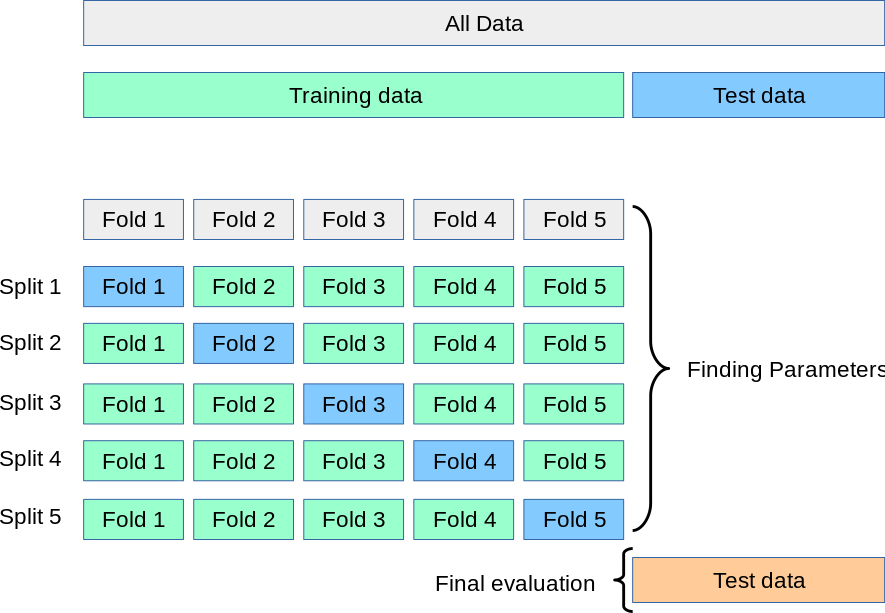
\includegraphics[scale=0.35]{k-fold}
		\caption{K-fold cross-validation scheme. The data is first split into train and test, and then the train is split again with this method \cite{Scikit-learna}}
		\label{fig:mesh16}
	\end{figure}

\chapter{Appendix Categorical cross-entropy}
\pagenumbering{gobble} 
\label{appendix:categorical-cross-entropy}

	In order to define this kind of loss function, it is necessary to consider the \textit{softmax} definition. As it was already explained in \ref{subsection:ann-cnn}, this function takes a vector and represents its elements in the range (0,1) as probabilities, so that all the resulting values must sum up to 1. In a multiclass classification, these are interpreted as class probabilities.
	
	These output probabilities can be evaluated with the cross-entropy loss. This is a way of measuring the performance of a model in which the output are probabilities between 0 and 1. The loss increases if the probability differs largely from the actual value of the true label. A perfect system would have a loss value of 0 \cite{MLGlossary2017}. In figure \ref{fig:mesh26}, an example of the loss function when the true label is 1 is shown.
	
	\begin{figure}[H]
		\centering
		\captionsetup{justification=centering}
		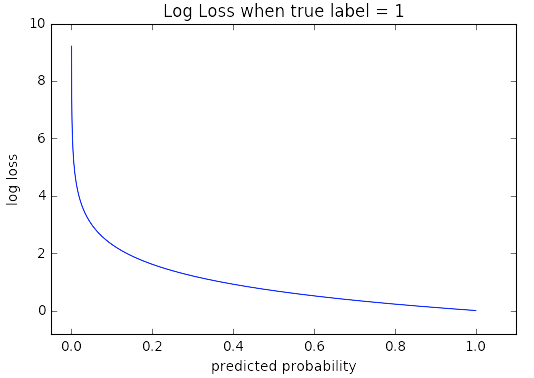
\includegraphics[scale=0.6]{ce}
		\caption{Cross-entropy loss function when the true label is equals to 1. As the probability of the predicted class approaches to 1, the loss function tends to zero. However, if it the probability is closer to 0.0, then the loss function increases heavily \cite{MLGlossary2017}.}
	\end{figure}

	Its formula is defined for binary problems as follows:
	
	\[
	\ CE = -(ylog(p) + (1 - y)log(1 - p))
	\]

	For a multiclass case, a unique loss is computed for each class label for each sample, and then the results are added as follows:
	
	\[
	\ CE = - \sum_{c=1}^{M} y_{o,c}log(p_{o,c})
	\]
	
	Where $M$ is the number of classes, $y$ is a indication in binary format if the class $c$ is the right prediction for this sample $o$ and $p$ is the estimation probability of $c$ for $o$ \cite{MLGlossary2017}. 
	
	Then, the categorical cross-entropy is a combination of softmax and the cross-entropy loss.
	
\chapter{Appendix Spectrogram and Mel scale}
\pagenumbering{gobble}
\label{appendix:spectrogram-mel-scale}

	In a natural situation the way humans understand audio as we hear it, can be interpreted as a succession of sounds that evolve with time. Actually, what happens during a recording process is that the signal registered is nothing but the variation of the values that represent the changes in the acoustic pressure along time, what is usually called the amplitude of the signal. This is what we see when visualizing a raw audio file in its original form, i.e. in the time-domain \cite{Laskaris2019}, as in figure \ref{fig:mesh49}.
	
	\begin{figure}[H]
		\centering
		\captionsetup{justification=centering}
		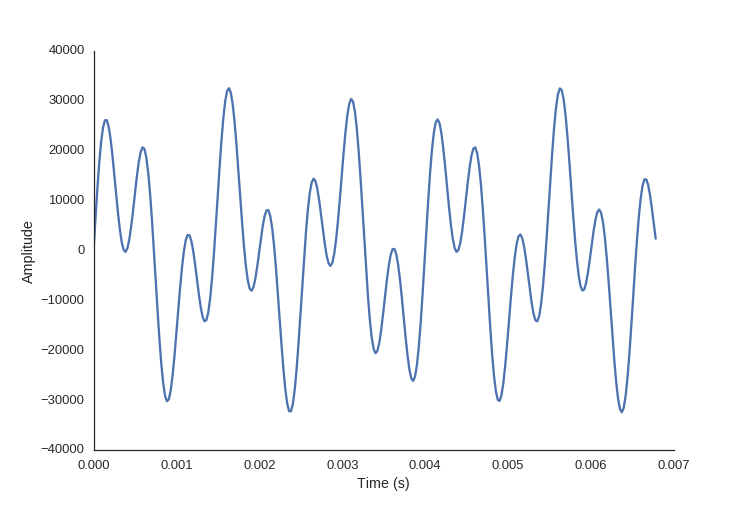
\includegraphics[scale=0.35]{time-signal}
		\caption{Audio signal in time domain}
		\label{fig:mesh49}
	\end{figure}

	However, in this form, audio data is not very useful for learning tasks. With the objective of representing audio data in another format so information can be extracted in a more practical way, it is normally converted to the frequency domain. The \acrshort{ft} is the technique in charge of performing this conversion. Since in signal processing we work with discrete data, the algorithm is called \acrfull{dft}, which is essentially the same as \acrshort{ft} but for discrete data and frequencies. The most common algorithm to compute this is the one called \acrfull{fft}, which performs the \acrshort{dft} in a more efficient way \cite{Lei2016}. The result of this method shows the values of the amplitude against the frequency axis. However, when the input is not stationary but it still can be regarded as such when observed within small portions, ther is also another method to perform this operation and it is called the \acrfull{stft}, which is the one used in this work.
	
	The \acrshort{stft} can be defined as a sequence of \acrshort{ft} s which are computed along a windowed signal. So, apart from computing the transformation, it also localizes in time this frequency information, given as a result a variation of the frequency along the time axis. Below, the formula of this operation is included:
	
	\[ X_{STFT} =  \sum_{k=0}^{L-1} x[k]g[k-m]e^{-j2\pi n k/L}\]
	
	$x[k]$ is the time signal of length $L$ and $g[k]$ is the window that goes through all the signal. In figure \ref{fig:mesh50}, a visualization of the whole process is shown \cite{Kehtarnavaz2008}.
	
	\begin{figure}[H]
		\centering
		\captionsetup{justification=centering}
		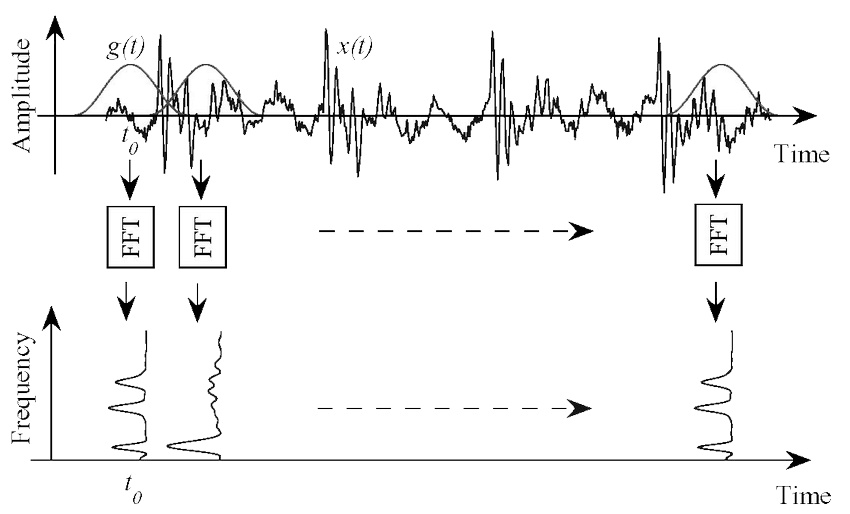
\includegraphics[scale=0.35]{stft}
		\caption{STFT \cite{Gao2006}}
		\label{fig:mesh50}
	\end{figure}

	What is obtained from this computation after transversing the whole signal, is a representation that depends on three magnitudes: time, frequency and the amplitude. This is known as the spectrogram of the signal. With this visualization we can see how the energy of the signal varies with time and also how it is placed in the different frequencies. In figure \ref{fig:mesh51} it is shown how a typical representation of a spectrogram looks like. 
	
	\begin{figure}[H]
		\centering
		\captionsetup{justification=centering}
		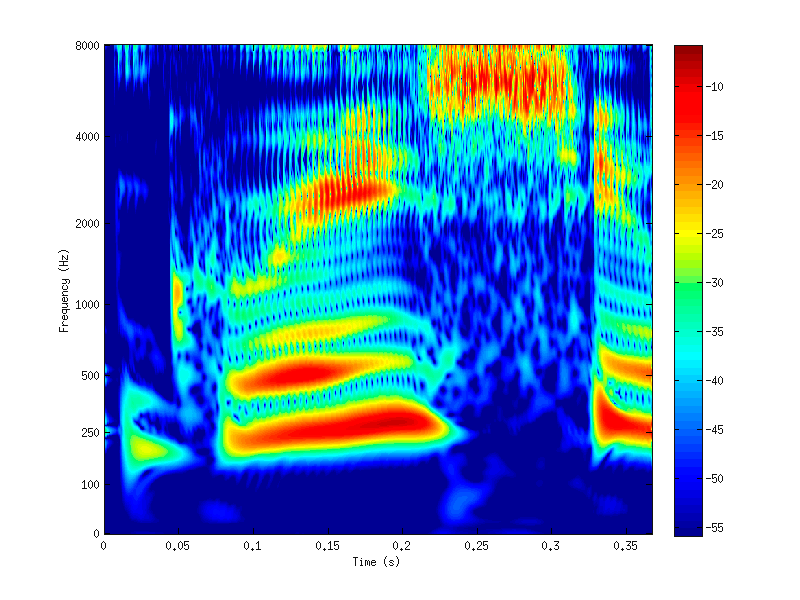
\includegraphics[scale=0.3]{spectrogram}
		\caption{Spectrogram of an audio signal. The x-axis corresponds to time, the y-axis to frequency and the colour of the plot to the amplitudes by following the colour bar on the right.}
		\label{fig:mesh51}
	\end{figure}

	When dealing with audio learning tasks we usually employ a logarithmic transformation of the frequency domain such as the Mel scale. %This is the result of applying a non-linear transformation to the frequency scale. 
	It has been successfully employed in plenty of applications because its similarities with how humans process sounds \cite{Gartzman2019}. This is done by considering the fact that we are more capable of differentiating small variations of pitch at low frequencies than at high ones. The following formula is the way to convert from frequency to mel scale \cite{Beranek1950}:
	
	\[M(f) = 1127 \ln{(1 + \frac{f}{700})}\]
	
	This same idea of applying the human way of understanding sounds has also been used to generate the \acrfull{mfcc}, which have been widely used in speech related problems. The first thing to understand in this area is that the sounds we produce by the lungs that make the vocal folds vibrate are subsequently filtered by the vocal tract. If a similar representation could be modelled in an artificial system, a more accurate depiction of the sound uttered could be achieved. Actually, the envelope of the short time power spectrum of the signal can be considered as the shape of this filter and it can be reliably represented by the \acrshort{mfcc}, so useful information can be deduced from them. This type of features have been extensively used for several fields such as automatic speech generation or speaker recognition but also in audio related ones \cite{Giannakopoulos2014}. 
	
	
	
	
	